\onecolumn
\section{Appendix}
% % Your table in single-column mode

\begin{figure}[h]
    \centering
    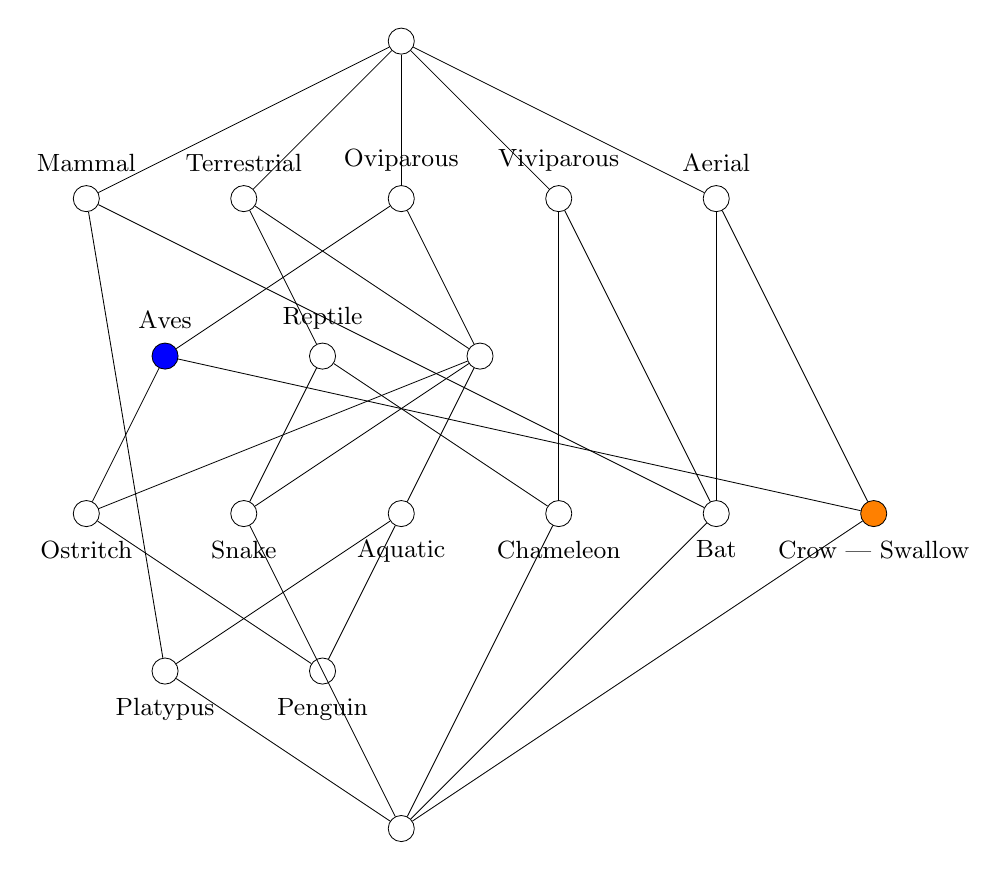
\begin{tikzpicture}[
            scale=1,
            concept/.style={circle, draw, line width=0.3pt, minimum size=0.2cm},
            label_above/.style={font=\small, above=0.05cm},
            label_below/.style={font=\small, below=0.05cm},
            line/.style={draw, line width=0.3pt}
        ]
        % Top node
        \node[concept] (root) at (0,8) {};

        % First level - characteristics
        \node[concept] (mammal) at (-4,6) {};
        \node[label_above] at (mammal.north) {Mammal};
        \node[concept] (terrestrial) at (-2,6) {};
        \node[label_above] at (terrestrial.north) {Terrestrial};
        \node[concept] (eggs) at (0,6) {};
        \node[label_above] at (eggs.north) {Oviparous};
        \node[concept] (young) at (2,6) {};
        \node[label_above] at (young.north) {Viviparous};
        \node[concept] (aerial) at (4,6) {};
        \node[label_above] at (aerial.north) {Aerial};

        % Middle level - classifications
        \node[concept,fill=blue] (aves) at (-3,4) {};
        \node[label_above] at (aves.north) {Aves};

        \node[concept] (mid_empty) at (1,4) {};

        \node[concept] (reptile) at (-1,4) {};
        \node[label_above] at (reptile.north) {Reptile};

        % Lower level
        \node[concept] (ostritch) at (-4,2) {};
        \node[label_below] at (ostritch.south) {Ostritch};
        \node[concept] (snake) at (-2,2) {};
        \node[label_below] at (snake.south) {Snake};
        \node[concept] (aquatic) at (0,2) {};
        \node[label_below] at (aquatic.south) {Aquatic};
        \node[concept] (chameleon) at (2,2) {};
        \node[label_below] at (chameleon.south) {Chameleon};
        \node[concept] (bat) at (4,2) {};
        \node[label_below] at (bat.south) {Bat};
        \node[concept,fill=orange] (crow) at (6,2) {};
        \node[label_below] at (crow.south) {Crow | Swallow};

        % Bottom level
        \node[concept] (platypus) at (-3,0) {};
        \node[label_below] at (platypus.south) {Platypus};
        \node[concept] (penguin) at (-1,0) {};
        \node[label_below] at (penguin.south) {Penguin};

        \node[concept] (bot) at (0,-2) {};

        \draw[line] (mammal) -- (root);
        \draw[line] (terrestrial) -- (root);
        \draw[line] (eggs) -- (root);
        \draw[line] (young) -- (root);
        \draw[line] (aerial) -- (root);

        \draw[line] (eggs) -- (aves);
        \draw[line] (eggs) -- (mid_empty);
        \draw[line] (terrestrial) -- (reptile);
        \draw[line] (terrestrial) -- (mid_empty);

        \draw[line] (mammal) -- (bat);
        \draw[line] (mammal) -- (platypus);

        \draw[line] (young) -- (bat);
        \draw[line] (young) -- (chameleon);

        \draw[line] (aerial) -- (bat);
        \draw[line] (aerial) -- (crow);

        \draw[line] (aves) -- (ostritch);
        \draw[line] (aves) -- (crow);

        \draw[line] (reptile) -- (snake);
        \draw[line] (reptile) -- (chameleon);

        \draw[line] (mid_empty) -- (snake);
        \draw[line] (mid_empty) -- (ostritch);
        \draw[line] (mid_empty) -- (aquatic);

        \draw[line] (crow) -- (bot);

        \draw[line] (ostritch) -- (penguin);

        \draw[line] (aquatic) -- (penguin);
        \draw[line] (aquatic) -- (platypus);

        \draw[line] (bat) -- (bot);

        \draw[line] (snake) -- (bot);

        \draw[line] (chameleon) -- (bot);

        \draw[line] (platypus) -- (bot);

    \end{tikzpicture}
    \caption{Concept lattice for the formal context in \cref{table: formal context}.}

    \label{figure: concept lattice}
\end{figure}

\begin{table}[h]
    \centering
    \begin{tabular}{rcccccccc}
                              & \texttt{Aves} & \texttt{Mammal} & \texttt{Reptile} & \texttt{Aerial} & \texttt{Aquatic} & \texttt{Terrestrial} & \texttt{Live Young} & \texttt{Eggs} \\
        \hline
        \texttt{Bat}          &               & $\times$        &                  & $\times$        &                  &                      & $\times$            &               \\
        \texttt{Crow}         & $\times$      &                 &                  & $\times$        &                  &                      &                     & $\times$      \\
        \texttt{Ostrich}      & $\times$      &                 &                  &                 &                  & $\times$             &                     & $\times$      \\
        \texttt{Penguin}      & $\times$      &                 &                  &                 & $\times$         & $\times$             &                     & $\times$      \\
        \texttt{Platypus}     &               & $\times$        &                  &                 & $\times$         & $\times$             &                     & $\times$      \\
        \texttt{Snake}        &               &                 & $\times$         &                 &                  & $\times$             &                     & $\times$      \\
        \texttt{Swallow}      & $\times$      &                 &                  & $\times$        &                  &                      &                     & $\times$      \\
        \texttt{J. Chameleon} &               &                 & $\times$         &                 &                  & $\times$             & $\times$            &               \\
    \end{tabular}
    \vspace{10pt}
    \caption{A formal context describing animals (objects) and some of their features (attributes)}
    \label{table: formal context}
\end{table}
\clearpage

% \twocolumn

% \begin{table}
% 	\centering
% 	\begin{tabular}{r|c|c|c|c|c|c|c|c|c|c}
% 		                   & \texttt{Aves} & \texttt{Mammal} & \texttt{Reptile} & \texttt{Aerial} & \texttt{Aquatic} & \texttt{Terrestrial} & \texttt{Migratory} & \texttt{Solitary} & \texttt{Carnivore} & \texttt{Eggs} \\
% 		\hline
% 		\texttt{Bat}       &               & $\times$        &                  & $\times$        &                  &                      &                    &                   & $\times$           &               \\
% 		\texttt{Crocodile} &               &                 & $\times$         &                 & $\times$         & $\times$             &                    &                   & $\times$           & $\times$      \\
% 		\texttt{Crow}      & $\times$      &                 &                  & $\times$        &                  &                      &                    &                   &                    & $\times$      \\
% 		\texttt{Hippo}     &               & $\times$        &                  &                 & $\times$         & $\times$             &                    & $\times$          &                    &               \\
% 		\texttt{Ostrich}   & $\times$      &                 &                  &                 &                  & $\times$             &                    & $\times$          &                    & $\times$      \\
% 		\texttt{Penguin}   & $\times$      &                 &                  &                 & $\times$         & $\times$             & $\times$           &                   & $\times$           & $\times$      \\
% 		\texttt{Platypus}  &               & $\times$        &                  &                 & $\times$         & $\times$             &                    & $\times$          & $\times$           & $\times$      \\
% 		\texttt{Snake}     &               &                 & $\times$         &                 &                  & $\times$             &                    & $\times$          & $\times$           & $\times$      \\
% 		\texttt{Swallow}   & $\times$      &                 &                  & $\times$        &                  &                      & $\times$           & $\times$          & $\times$           & $\times$      \\
% 		\texttt{Whale}     &               & $\times$        &                  &                 & $\times$         &                      & $\times$           & $\times$          & $\times$           &               \\
% 	\end{tabular}
% 	\caption{Cross-table of $\K$}
% 	\label{tab:formal-context}
% \end{table}


% \begin{algorithm}
% 	\caption{Computing the tolerance partition on objects $G$}
% 	\begin{algorithmic}[1]
% 		\Require A formal context, $\FC$;
% 		\Require A set of defeasible implications, $\Delta$;
% 		\Ensure A tolerance partition $(R_0, \ldots, R_n)$ on $G$;
% 		\State $P_0 \gets G$;
% 		\State $i \gets 0$;
% 		\State $\Delta \gets \text{Material} (\Delta)$;
% 		\While {$P_{i-1} \neq P_i}$
% 			\State $P_{i+1} \gets \{g \in P_i \mid \exists \delta \in \Delta  g' \st g'\not \models \delta \}$;
% 			\State $R_i \gets P_i \setminus P_{i+1}$;
% 			\State $\Delta_i \gets \{ (\alpha \rightarrow \beta) \in \Delta \mid \exists g \in P_i \st \alpha \subseteq g'\}$;
% 			\State $\Delta \gets \Delta \setminus \Delta_i$;
% 			\EndWhile
% 			\If {$P_{i-1} = \emptyset$}
% 			\State $n \gets i-1$;
% 			\Else
% 			\State $n \gets i$;
% 			\EndIf
% 			\State \Return $\big (R_0,\ldots, R_n \big)$;
% 	\end{algorithmic}
% \end{algorithm}

% To clarify some points on
% \begin{itemize}
% 	\item Line $3$: this step turns $\Delta$ into a set of material implications;
% 	\item Line $5$: this step puts into ranking $i+1$ every object which \textbf{does not} respect $\Delta$;
% 	\item Line $7$: this sets $\Delta_i$ to be the set of formulae in $\Delta$ which have their antecedent satisfied by an object in $P_i$ (implicitly all objects in $P_i$ satisfy all formulae in $\Delta$, but we only care about the ones which have their antecedent satisfied);
% 	\item We update $\Delta$ to be those formulae which are not yet ``dealt with''.
% \end{itemize}

% \begin{algorithm}
% 	\caption{Checking entailment}
% 	\begin{algorithmic}[1]
% 		\Require A formal context, $\FC$;
% 		\Require A set of defeasible implications, $\Delta$;
% 		\Ensure A tolerance partition $(R_0, \ldots, R_n)$ on $G$;
% 		\State $P_0 \gets G$;
% 		\State $i \gets 0$;
% 		\State $\Delta \gets \text{Material} (\Delta)$;
% 		\While {$P_{i-1} \neq P_i}$
% 			\State $P_{i+1} \gets \{g \in P_i \mid \exists \delta \in \Delta  g' \st \not \Vdash \delta \}$;
% 			\State $P_i \gets P_i \setminus P_{i+1}$;
% 			\State $\Delta_i \gets \{ (\alpha \rightarrow \beta) \in \Delta \mid \exists g \in P_i \st \alpha \subseteq g'\}$;
% 			\State $\Delta \gets \Delta \setminus \Delta_i$;
% 			\EndWhile
% 			\If {$P_{i-1} = \emptyset$}
% 			\State $n \gets i-1$;
% 			\Else
% 			\State $n \gets i$;
% 			\EndIf
% 			\State \Return $\big (P_0,\ldots, P_n \big)$;
% 	\end{algorithmic}
% \end{algorithm}
% \clearpage
\small
\subsection{Risks}
\label{appendix: risks}

\begin{table}[!ht]
    \begin{tabularx}{\linewidth}{>{\justifying\arraybackslash}X>{\centering\arraybackslash}p{2cm}>{\centering\arraybackslash}p{2cm}>{\justifying\arraybackslash}X>{\justifying\arraybackslash}X>{\justifying\arraybackslash}X}
        \hline
        \textbf{Risk Description}                                                                                         & \textbf{Probability} & \textbf{Impact} & \textbf{Mitigation}                                                                                                                                                                                                & \textbf{Monitor}                                                                                            & \textbf{Manage}                                                                                                                                                                      \\
        \hline
        Not being able to achieve the research goals I set out to, (i.e. showing it cannot be done, or failing otherwise) & $0.4$                & $0.5$           & Ensure realistic goals, and that each phase of research is scrutinised to avoid realising error much later on                                                                                                      & Keep track of progress                                                                                      & In case of showing this method does not work, recognition that positive results are not necessarily required. Otherwise, consult with supervisors on how the scope may be redefined. \\
        Novel contributions of my work are published elsewhere beforehand                                                 & $0.2$                & $0.3$           & Ensure that I try publish results as soon as it is ready. Pay attention to upcoming conferences and submission dates.                                                                                              & Make sure I keep up to date with FCA publications to observe research trends.                               & Since this work is a MSc, there is no requirement for novelty. Ensure that I mention these results alongside my own.                                                                 \\
        Problem is too difficult/I get stuck on something.                                                                & $0.4$                & $0.2$           & Ensure frequent discussion with supervisors and lab-mates, asking for help when things are not clear. In addition, refer back to foundational texts to make sure my understanding of the broader field(s) is good. & A sign of not understanding things fully would be frequently making errors; monitor work for signs of this. & If I reach a point where I am not understanding the work, go back to the last point where I feel a solid grasp of the concepts, and move forward slowly.                             \\
        Suffering from fatigue, or burnout.                                                                               & $0.4$                & $0.6$           & Ensure I develop a healthy work routine, which allows me to do things outside of work, while easing fears that I'm not doing enough.                                                                               & Generally check-up on myself.                                                                               & If I do begin to feel like this, speak to supervisors about taking a short break, and then return to work later on.                                                                  \\
        Loss of work/material due to technical issues.                                                                    & $0.1$                & $0.8$           & Ensure all digital work is backed up to secure location, written work should be copied and digitised.                                                                                                              & -                                                                                                           & If this does happen, make attempts to recover lost files. Otherwise, reconstruct lost work.                                                                                          \\
        Writing/documentation challenges                                                                                  & $0.4$                & $0.3$           & Start writing early. Break thesis into manageable sections. Maintain good research notes from day one.                                                                                                             & Ensure I do regular progress checks. Keep track of references and sources properly.                         & Seek writing support if needed. Consider writing workshops or peer review groups.                                                                                                    \\
    \end{tabularx}
\end{table}

\subsection{Deliverables}
\label{appendix: deliverables}
\begin{table}[!ht]
    \begin{tabularx}{\linewidth}{>{\justifying\arraybackslash}X>{\centering\arraybackslash}p{2cm}>{\centering\arraybackslash}p{2cm}>{\justifying\arraybackslash}X}
        \hline
        \textbf{Task}                        & \textbf{Start} & \textbf{End} & \textbf{Comments}                                                               \\
        \hline
        Proposal                             & 05.10.24       & 28.10.24     & Submit draft one week before deadline                                           \\
        Background Thesis Chapters           & 01.11.24       & 31.01.25     & Submit rough outlines, and semi-incremental updates for review before deadline. \\
        Novel Results Write-Up               & 01.02.25       & 31.04.25     & While this process occurs, have meetings/feedback sessions.  results            \\
        Thesis Consolidation                 & 01.05.25       & 31.06.25     & This should be a more-or-less finished document.                                \\
        Final Review and Intention to Submit & 01.07.25       & 31.07.25     & Final adjustments and corrections                                               \\
    \end{tabularx}
\end{table}

\clearpage
\subsection{Gantt Chart}
\label{appendix: gantt chart}
\begin{table}[!ht]

    \rotatebox{270}{
        % \parbox{25cm}{
        \begin{tabular}{rlllllllllllllllllllllllllllllllllllllll}
            \textbf{2024}                  & ~     & ~     & ~     & ~     & ~     & ~     & ~     & ~     & ~     & \textbf{2025} & ~     & ~     & ~     & ~     & ~     & ~     & ~     & ~      \\
            ~                              & April & May   & June  & July  & Aug   & Sept  & Oct   & Nov   & Dec   & Jan           & Feb   & March & April & May   & June  & July  & Aug   & Sept.. \\
            ~                              & ~     & ~     & ~     & ~     & ~     & ~     & ~     & ~     & ~     &               &       &       &       &       &       &       &       &        \\
            \textbf{Literature Engagement} & \ccbM & \ccbM & \ccbM & \ccbM & \ccbM & \ccbM & \ccbM & \ccbM & \ccbM & \ccbM         & \ccbM &       &       &       &       &       &       &        \\
            \textbf{Learning}              & \ccbM & \ccbM & \ccbM & \ccbM & \ccbM &       & \ccbM & \ccbM & \ccbM & \ccbM         & \ccbM & \ccbM &       &       &       &       &       &        \\
            Learning FCA                   & ~     & \ccbS & \ccbS & ~     & \ccbS & ~     & ~     & \ccbS & ~     &               &       &       &       &       &       &       &       &        \\
            Learning KLM                   & \ccbS & ~     & \ccbS & \ccbS & \ccbS & ~     & \ccbS & ~     & ~     &               &       &       &       &       &       &       &       &        \\
            Lattice Theory + Misc          & ~     & ~     & \ccbS &       & ~     & ~     & ~     & \ccbS & \ccbS & \ccbS         &       &       &       &       &       &       &       &        \\
            \textbf{Development}           & \ccbM & \ccbM & \ccbM & \ccbM & \ccbM & \ccbM & \ccbM & \ccbM & \ccbM & \ccbM         & \ccbM & \ccbM &       &       &       &       &       &        \\
            Developing questions           & \ccbS & ~     & \ccbS & ~     & \ccbS & ~     & ~     & \ccbS & ~     &               &       & \ccbS &       &       &       &       &       &        \\
            Investigating questions        & ~     & \ccbS & ~     & \ccbS & ~     & \ccbS & \ccbS & \ccbS & \ccbS & \ccbS         & \ccbS &       &       &       &       &       &       &        \\
            \textbf{Thesis Writing}        &       &       &       &       &       &       &       &       & \ccbM & \ccbM         & \ccbM & \ccbM & \ccbM & \ccbM & \ccbM &       &       &        \\
            FCA Background                 &       &       &       &       &       &       &       &       & \ccbS &               & \ccbS &       &       &       &       &       &       &        \\
            NMR Background                 &       &       &       &       &       &       &       &       & \ccbS & \ccbS         & \ccbS &       &       &       &       &       &       &        \\
            Defeasible Implications        &       &       &       &       &       &       &       &       &       &               & \ccbS & \ccbS & \ccbS &       &       &       &       &        \\
            Rational Concepts              &       &       &       &       &       &       &       &       &       &               & \ccbS & \ccbS & \ccbS &       &       &       &       &        \\
            Consolidation                  &       &       &       &       &       &       &       &       &       &               &       &       &       & \ccbS & \ccbS & \ccbS &       &        \\
            Submit                         &       &       &       &       &       &       &       &       &       &               &       &       &       &       &       &       & \ccbS &        \\
            Proposal                       &       &       &       &       &       &       & \ccbS &       &       &               &       &       &       &       &       &       &       &        \\
            Publish second paper           &       &       &       &       &       &       &       &       &       &               &       & \ccbS & \ccbS & \ccbS & \ccbS &       &       &        \\
            \textbf{Events}                & \ccbM & \ccbM & \ccbM & \ccbM & \ccbM & \ccbM &       &       & \ccbM &               & \ccbM &       & \ccbM & \ccbM & \ccbM & \ccbM &       &        \\
            Dresden                        & \ccbS & \ccbS & \ccbS & \ccbS &       &       &       &       &       &               &       &       &       &       &       &       &       &        \\
            SACAIR                         &       &       &       &       & \ccbS & \ccbS &       &       &       &               &       &       &       &       &       &       &       &        \\
            Paper Writing                  &       &       &       &       & \ccbS & \ccbS &       &       &       &               &       &       &       &       &       &       &       &        \\
            Paper Edits                    &       &       &       &       &       &       & \ccbS &       &       &               &       &       &       &       &       &       &       &        \\
            Conference                     &       &       &       &       &       &       &       &       & \ccbS &               &       &       &       &       &       &       &       &        \\
            Cape KR                        &       &       &       &       &       &       &       &       &       &               & \ccbS &       &       &       &       &       &       &        \\
            Semester in paris              &       &       &       &       &       &       &       &       &       &               &       &       & \ccbS & \ccbS & \ccbS & \ccbS &       &
        \end{tabular}
        % \vspace{1cm}
        % \caption{\textcolor[HTML]{b6bfdb}{Blue} indicates main task, while \textcolor[HTML]{b6dbb7}{green} indicates sub-task}
        % }
    }

    \caption{\textcolor[HTML]{b6bfdb}{Blue} indicates main task, while \textcolor[HTML]{b6dbb7}{green} indicates sub-task}
\end{table}
